\documentclass[10pt,a4paper]{article}
\usepackage[utf8]{inputenc}
\usepackage[spanish]{babel}
\usepackage{amsmath}
\usepackage{amsfonts}
\usepackage{amssymb}
\usepackage{graphicx}
\usepackage[left=2cm,right=2cm,top=2cm,bottom=2cm]{geometry}
\usepackage{listings}
\usepackage[hidelinks]{hyperref}

% Frame over lstlisting
\lstset { frame = single }


\begin{document}

\begin{titlepage}
\title{\textbf{
	{\Huge SELinux}\\
	{\Large Seguridad Informática}
}}
\author{
	Pedro Allué Tamargo (758267)
	\and
	Juan José Tambo Tambo (755742)
}
\date{\today}
\clearpage\maketitle
\thispagestyle{empty}
\tableofcontents
\end{titlepage}

\section{Parte 1: Información, estado y dominios en \emph{SELinux}}

Tras iniciar sesión con el usuario \emph{u} se ejecuta el comando \texttt{ps aux} y se puede observar en la salida del comando que los usuarios efectivos que están ejecutando procesos en el sistema son: \emph{root, dbux, rpc, rpcuser, 68, postfix, gdm, rtkit, u}.\\

Si ejecutamos el comando \texttt{ps auxZ} se puede observar que una salida similar a la del comando anterior pero con la diferencia de que aparecen los usuarios, roles y dominios \emph{SELinux} de los procesos en ejecución en el sistema.\\

Los usuarios \emph{Linux} que están ejecutando procesos en dominios \texttt{unconfined\_{}t} son: \emph{u}.\\
Los usuarios \emph{Linux} que están ejecutando procesos con el usuario y rol \texttt{system\_{}u :system\_{}r} son: \emph{root, rpc, rpcuser, 68, postfix, gdm, rtkit}.\\
La diferencia entre que unos procesos están en dominios \texttt{unconfined\_{}t} y otros no radica en que los procesos con dominio \texttt{unconfined\_{}t} se corresponde con los ejecutados por un usuario \emph{logged-in} (usuario \emph{u}), mientras que el resto se corresponden con procesos ejecutados por usuarios que no han iniciado sesión en el sistema.\\

Si se invoca el comando \texttt{passwd} en otra terminal se puede observar que el usuario \emph{Linux} del proceso se corresponde con el usuario \emph{root} ya que el binario \emph{passwd} tiene el bit \emph{setuid} activo. También se puede observar que el usuario y el rol del proceso sigue siendo \texttt{unconfined\_{}u:unconfined\_{}r} pero el dominio del proceso ha cambiado \texttt{passwd\_{}t}. Esto se debe a que se ha producido una transición de dominio en el cual se ha sustituido \texttt{unconfined\_{}t} por \texttt{passwd\_{}t}.\\

La interacción con \emph{SELinux} no es solo mediante línea de comandos, también se puede interactuar utilizando la herramienta gráfica \emph{SELinux Manage} (Figura \ref{fig:parte1_5a}) disponible en el sistema. Esta herramienta utiliza la interfaz de línea de comandos y muestra la información de una forma más ``amigable'' para el usuario.\\

\begin{figure}[h!]
\centering
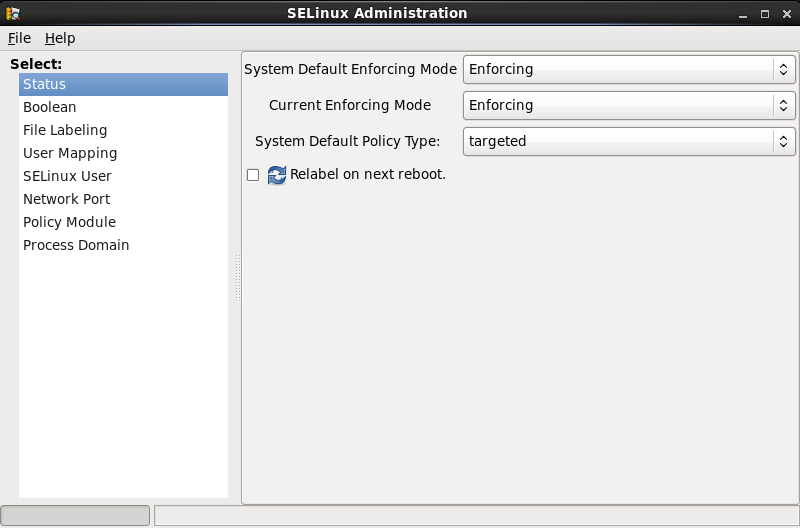
\includegraphics[scale=0.5]{images/parte1_5a.png}
\caption{Captura de pantalla de la aplicación gráfica}
\label{fig:parte1_5a}
\end{figure}

Por ejemplo en el apartado \emph{``User Mapping''} (Figura \ref{fig:parte1_5b}) se puede observar la relación entre los usuarios de \emph{Linux} y los usuarios de \emph{SELinux}. Esto también se puede observar utilizando el comando \texttt{semanage login -l} (Figura \ref{fig:parte1_5d}).\\

\begin{figure}[h!]
\centering
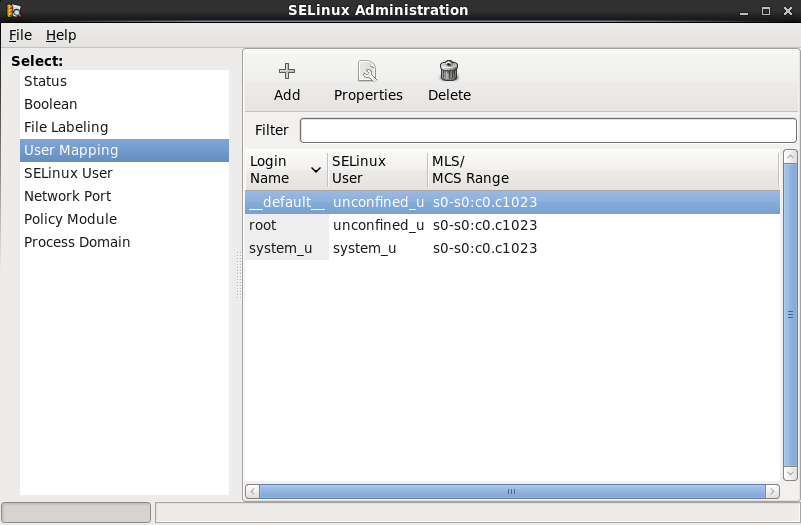
\includegraphics[scale=0.5]{images/parte1_5b.png}
\caption{Captura de pantalla del apartado \emph{``User Mapping''}}
\label{fig:parte1_5b}
\end{figure}

\begin{figure}[h!]
\centering
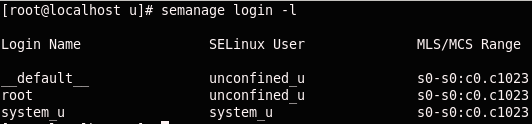
\includegraphics[scale=0.5]{images/parte1_5d.png}
\caption{Captura de pantalla de la salida del comando \texttt{semanage login -l}}
\label{fig:parte1_5d}
\end{figure}

\newpage
\section{Parte 2: Usuarios en \emph{SELinux}}

Se va a proceder a crear un nuevo usuario \emph{c}. Para ello se utilizará el comando \texttt{adduser -Z user\_{}u c}. Este comando creará el usuario \emph{Linux} \texttt{c} y el usuario \emph{SELinux} \texttt{user\_{}u}.\\
Tras la creación del usuario se cambiará al usuario \emph{c} (\texttt{su - c}) y se ejecutará el comando \texttt{id}. La salida de este comando (Figura \ref{fig:parte2_7}) muestra en el apartado del contexto la cadena: \texttt{unconfined\_{}u:unconfined\_{}r:unconfined\_{}t}. Esto muestra que el usuario \emph{c} se corresponde con el usuario de \emph{SELinux} \texttt{unconfined\_{}u}. Esto no es completamente cierto. En la creación del usuario de \emph{Linux} \emph{c} se le ha asignado al usuario de \emph{SELinux} \texttt{user\_{}u}, pero al haber realizado el login con el usuario \emph{u} se han mantenido su usuario, rol y tipo de \emph{SELinux}.\\

\begin{figure}[h!]
\centering
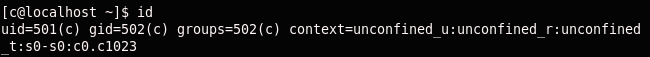
\includegraphics[scale=0.5]{images/parte2_7.png}
\caption{Captura de pantalla de la salida del comando \texttt{id} con el usuario \emph{c}}
\label{fig:parte2_7}
\end{figure}

Si se ejecuta la orden \texttt{semanage login -l} (Figura \ref{fig:parte2_8}) se puede observar que el usuario \emph{u} no existe y aparece una entrada en la tabla para el usuario \emph{c} que asocia ese usuario de \emph{Linux} con el usuario \emph{SELinux} \texttt{user\_{}u}.

\begin{figure}[h!]
\centering
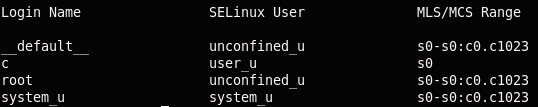
\includegraphics[scale=0.5]{images/parte2_8.png}
\caption{Captura de pantalla de la salida del comando \texttt{semanage login -l}}
\label{fig:parte2_8}
\end{figure}

Si iniciamos sesión en la interfaz gráfica con el usuario \emph{c} y volvemos a ejecutar el comando \texttt{id} en una terminal se obtendrá la salida mostrada en la Figura \ref{fig:parte2_10}. Se puede observar que ha cambiado el contexto (usuario, rol y tipo de \emph{SELinux}) y ahora muestra la siguiente información \texttt{user\_{}u:user\_{}r:user\_{}t}.\\

\begin{figure}[h!]
\centering
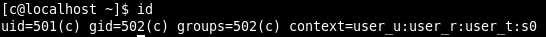
\includegraphics[scale=0.7]{images/parte2_10.png}
\caption{Captura de pantalla de la salida del comando \texttt{id} con el usuario \emph{u}}
\label{fig:parte2_10}
\end{figure}

Ahora utilizando al usuario \emph{c} se va a intentar ejecutar el comando \texttt{su -} para acceder a la cuenta \emph{root}. El resultado es que no se puede utilizar este binario (\texttt{su}) ya que en \emph{SELinux} hay que proveer permisos explícitos para permitir ciertas acciones, en este caso ejecutar un fichero que no pertenece al dominio \texttt{bin\_{}t}. Este binario (Figura \ref{fig:parte2_11}) pertenece al dominio \texttt{su\_{}exec\_{}t}. Para poder utilizar este binario habrá que crear una regla de acceso que relacione el tipo \texttt{user\_{}t} con el dominio \texttt{su\_{}exec\_{}t}. La regla de acceso tendría la forma:

\begin{lstlisting}
allow user_t su_exec_t:file {read execute getaddr};
\end{lstlisting}

\begin{figure}[h!]
\centering
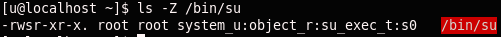
\includegraphics[scale=0.7]{images/parte2_11.png}
\caption{Captura de pantalla de la salida del comando \texttt{ls -Z /bin/su}}
\label{fig:parte2_11}
\end{figure}

\section{Parte 3: Listas de Control de Accesos (\emph{ACLs}) basados en estándar \emph{POSIX} de \emph{Unix} del modelo \emph{DAC}}



\section{Parte 4: Reglas de control de accesos y acceso a dominios}




\end{document}